\documentclass[dvipsnames, tikz]{standalone}
\usepackage{amsmath}
\usepackage{arevmath}
\usepackage{xcolor}
\usepackage{tikz}
\usetikzlibrary{calc}
\usetikzlibrary{decorations.pathreplacing,calligraphy,3d}
\usetikzlibrary{matrix,shapes,fit,backgrounds}

\begin{document}
	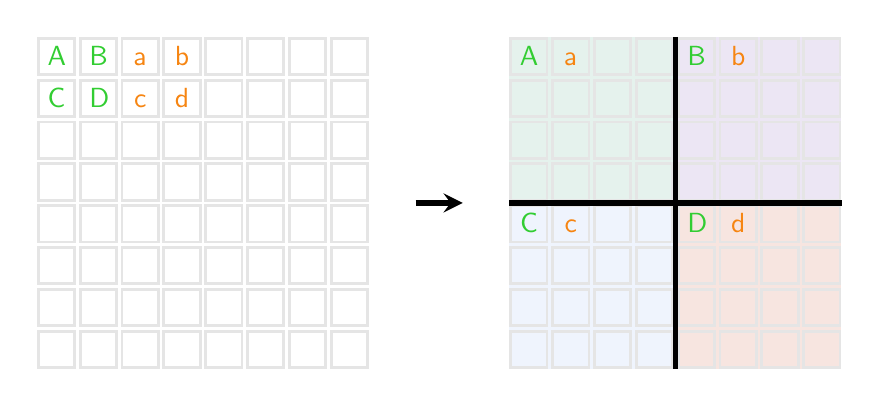
\begin{tikzpicture}[
		%Global config
		>=latex,
		line width=1pt,
		color = black,
		every left delimiter/.style={xshift=1ex},
		every right delimiter/.style={xshift=-1ex},
		%Styles
		Matrix/.style={
			matrix of nodes,
			text height=1.5ex,
			%text depth=0.75ex,
			text width=1.5ex,
			align=center,
			%left delimiter=(,
			%right delimiter=),
			column sep=1pt,
			row sep=1pt,
			nodes={draw=black!10}, % Uncoment to see the square nodes.
			nodes in empty cells,
		},
		DA/.style={
			fill,
			opacity=0.2,
			%rounded corners,
			inner sep=0pt,
			line width=1pt,
		},
		main/.style={
			line width=2pt,
			color=black
		},
		DG/.style={
			line cap = round,
			rounded corners=0.25ex,
			line width = 8pt,
			opacity = 0.3,
		}
		]
		
		\matrix[Matrix] at (0,0) (M){ % Matrix contents  
			\sf \color{LimeGreen}A & \sf \color{LimeGreen}B & \sf \color{BurntOrange}a&  \sf \color{BurntOrange}b&  \null& \null &\null & \null \\
			\sf \color{LimeGreen}C & \sf \color{LimeGreen}D & \sf \color{BurntOrange}c&  \sf \color{BurntOrange}d&  \null& \null &\null & \null \\
			\null & \null &  \null&  \null&  \null& \null &\null & \null \\
			\null & \null &  \null&  \null&  \null& \null &\null & \null \\
			\null & \null &  \null&  \null&  \null& \null &\null & \null \\
			\null & \null &  \null&  \null&  \null& \null &\null & \null \\
			\null & \null &  \null&  \null&  \null& \null &\null & \null \\
			\null & \null &  \null&  \null&  \null& \null &\null & \null \\
		};
	
		\matrix[Matrix] at (6,0) (M){ % Matrix contents  
			\sf \color{LimeGreen}A & \sf \color{BurntOrange}a & \null & \null & \sf \color{LimeGreen}B & \sf \color{BurntOrange}b &\null & \null \\
			\null & \null &  \null&  \null&  \null& \null &\null & \null \\
			\null & \null &  \null&  \null&  \null& \null &\null & \null \\
			\null & \null &  \null&  \null&  \null& \null &\null & \null \\
			\sf \color{LimeGreen}C & \sf \color{BurntOrange}c &  \null&  \null&  \sf \color{LimeGreen}D& \sf \color{BurntOrange}d &\null & \null \\
			\null & \null &  \null&  \null&  \null& \null &\null & \null \\
			\null & \null &  \null&  \null&  \null& \null &\null & \null \\
			\null & \null &  \null&  \null&  \null& \null &\null & \null \\
		};
		
		\draw[main] (3.89,0) --++ (4.22,0);
		
		\draw[main] (6,2.11) --++ (0,-4.22);
		
		\begin{scope}[on background layer] 
			%To delimit internal area groups
			\node[DA,PineGreen!50,fit=(M-1-1)(M-4-4)](subM-1){};
			\node[DA,RoyalPurple!50,fit=(M-1-5)(M-4-8)](subM-2){};
			\node[DA,CornflowerBlue!50,fit=(M-5-1)(M-8-4)](subM-3){};
			\node[DA,BrickRed!50,fit=(M-5-5)(M-8-8)](subM-4){};
			
			\draw[main, -stealth] (2.7,0) --++ (0.6,0);
			
			
			
			% For line sectors
			%\draw[DG,LimeGreen](M-1-1.center) --(M-1-3.center) --(M-3-3.center)--(M-3-1.center)--(M-2-1.center)--(M-2-2.center);
		\end{scope}
	\end{tikzpicture}
\end{document}